\documentclass[titlepage]{article}
\usepackage{textcomp}
\usepackage{float}
\usepackage{listings}
\usepackage{fancyhdr}
\usepackage{tikz}
\usepackage{pgfplots}

\lstset{breaklines=true}
\pgfplotsset{compat=1.15}

\title{EECS 690 Project 2}
\author{Zane J Cersovsky}
\fancyhf{}
\pagestyle{fancy}
\renewcommand{\headrulewidth}{0pt}
\lfoot{\textcopyright 2017 Zane J Cersovsky}
\cfoot{\thepage}

\tikzstyle{block} = [draw, rectangle, minimum height=2em, minimum width=4em]

\begin{document}

\maketitle

\section{Abstract} 
The purpose of this project was to design one or more laboratory exercises targeting the Texas Instruments EK-TM4C1294XL
evaluation board (``Tiva\textregistered'' for short) that could be performed by a student in EECS 388. As such, one of 
the key parts of this project was to design a suitable abstraction layer that would hide enough of the implementation 
details of hardware interaction to allow focus to remain on the exercise but would not do too much and take away 
content from the lab.

Once the abstraction layer was designed, three laboratory exercises were designed that, in the spirit of the current 
EECS 388 labs, progressively built upon on each other with one new piece of hardware/concept added each time. The first lab 
mimics the current 388 lab 02 as closely as possible (making a single tone with a speaker using unreliable timing). The second 
lab has the same end result as the first, but has timing derived from a hardware timer and interrupt service routine. The 
lab uses a combination of the first two, with the tone generated by an ISR but varied by a task to show, among other things, 
a way to use floating-point on the Tiva\textregistered.

For extra flexibility, none of the labs were designed with a hard dependency on FreeRTOS\textregistered, but have sample 
implementations using it. In addition, extra time was available, so there is an extra sample included that generates a 
sine wave in place of the square wave generated by three labs present in the original design.

\pagebreak
\tableofcontents
\pagebreak
\listoffigures
\pagebreak
\listoftables
\pagebreak

\section{Principles of Operation}
\paragraph{Summary}
Each laboratory exercise relies on a set of drivers designed and implemented especially for this project. From highest-
level to lowest, these are: the Audio BoosterPack\textregistered\space driver, the DAC8311 driver, and the SPI Master driver. 
Each one of these drivers uses and extends the one below it to add an abstraction layer. Each driver initializes any hardware 
that it needs. This is a deviation from the original design in which only the BoosterPack\textregistered\space driver initialized 
hardware. Early on in the implementation phase, it became very apparent that this would result in a very large BoosterPack\textregistered\space
driver and nearly-meaningless SPI and DAC drivers.
\begin{figure}[H]
    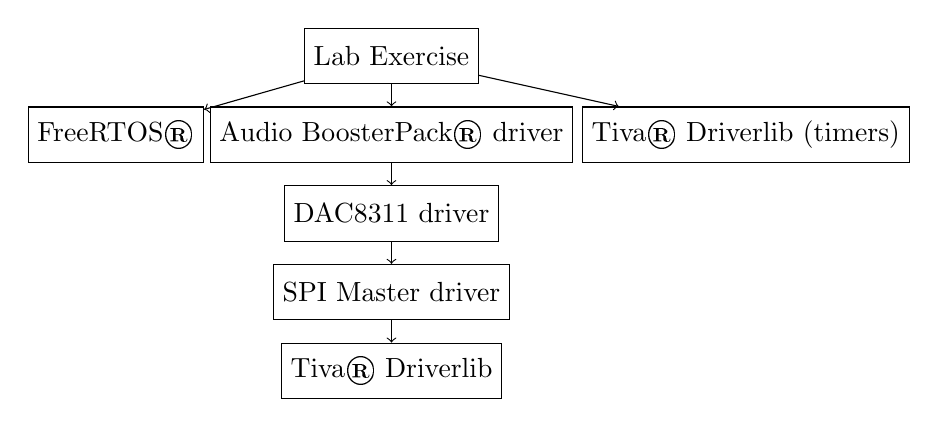
\begin{tikzpicture}
        \node[block] (lab) {Lab Exercise};
        \node[block] (booster) [below of=lab] {Audio BoosterPack\textregistered\space driver};
        \node[block] (freertos) [left of=booster, node distance=3.5cm] {FreeRTOS\textregistered};
        \node[block] (timers) [right of=booster, node distance=4.5cm] {Tiva\textregistered\space Driverlib (timers)};
        \node[block] (dac) [below of=booster] {DAC8311 driver};
        \node[block] (spi) [below of=dac] {SPI Master driver};
        \node[block] (driverlib) [below of=spi] {Tiva\textregistered\space Driverlib};
        \draw[->] (lab) edge (freertos);
        \draw[->] (lab) edge (booster);
        \draw[->] (lab) edge (timers);
        \draw[->] (booster) edge (dac);
        \draw[->] (dac) edge (spi);
        \draw[->] (spi) edge (driverlib);
    \end{tikzpicture}
    \caption{Laboratory Exercise Architecture}
\end{figure}

\paragraph{Audio BoosterPack\textregistered driver}
This driver is very simple: in its present state, it only initializes the necessary hardware and other drivers and then 
passes through the write method from the DAC driver. It was intended to provide a good place to collect all of the 
hardware initialization tasks and provide a place to make other abilities of the BoosterPack\textregistered available. In 
the future, this could include the microphone.

\paragraph{DAC8311 driver}
This driver encapsulates the logic needed for writing a value to the DAC. For each value, it must be enforced that the 
value is 16 bits long with the highest two bits set to $00$. The first property reflects the word length of the DAC and is 
enforced by the argument type of the \texttt{DAC8311Write} method. The second is due to the DAC8311 using the high two 
bits for power control. Values other than $00$ represent various power-down states.

\paragraph{SPI Master driver}
This driver is responsible for initializing the SSI (SPI) and GPIO hardware in the microcontroller and writing words. This 
is mostly a wrapper around the Tivaware\textregistered\space driver, but specialized only for legacy SPI (i.e. no multi-wire advanced 
mode support). Originally, it was planned that this would include a way to write entire buffers, but using the $\mu$DMA engine is 
a much better option for that task.

\pagebreak
\section{Data Structure Descriptions}

\begin{figure}[H]
\begin{lstlisting}
struct AudioInst {
    struct SPIInstance spim;
    struct DAC8311Instance dac;
};
\end{lstlisting}
\caption{Audio BoosterPack\textregistered\space instance data}
\end{figure}

\begin{figure}[H]
\begin{lstlisting}
struct DAC8311Instance {
    struct SPIInstance* spim;
};
\end{lstlisting}
\caption{DAC8311 driver instance data}
\end{figure}

\begin{figure}[H]
\begin{lstlisting}
struct SPIInstance {
    void* base_addr;
    enum SPIProtocol protocol; //polarity and phase info
};
\end{lstlisting}
\caption{SPI Master driver instance data}
\end{figure}

\pagebreak
\section{Function Descriptions}

\subsection{AudioPack.c}

\paragraph{AmpEnable}
\subparagraph{Description}
Enables the amplifier present on the Audio BoosterPack\textregistered.
\begin{figure}[H]
    \begin{verbatim}
ENABLE GPIO Port P
SET Port P, Pin 3 to Low
    \end{verbatim}
    \caption{Pseudocode for AmpEnable}
\end{figure}

\paragraph{AudioInit}
\subparagraph{Description}
Initializes the hardware and software needed to use the Audio BoosterPack\textregistered.
\begin{figure}[H]
    \begin{verbatim}
CALL AmpEnable
INIT SPI Master driver with the correct settings
INIT DAC8311 driver with the correct settings
    \end{verbatim}
    \caption{Pseudocode for AudioInit}
\end{figure}

\paragraph{DACWrite}
\subparagraph{Description}
Wraps the DAC driver write method.
\begin{figure}[H]
    \begin{verbatim}
CALL DAC8311Write with the instance held by this driver, $value
    \end{verbatim}
    \caption{Pseudocode for DACWrite}
\end{figure}

\subsection{DAC8311.c}

\paragraph{DAC8311Init}
\subparagraph{Description}
Initializes the DAC8311 driver
\begin{figure}[H]
    \begin{verbatim}
STORE the provided SPI instance into the instance of this driver
    \end{verbatim}
    \caption{Pseudocode for DAC8311Init}
\end{figure}

\paragraph{DAC8311Write}
\subparagraph{Description}
Writes a single value to the DAC8311
\begin{figure}[H]
    \begin{verbatim}
SET the two most significant bits of the $value
CALL SPIMWriteWord with the instance held by this driver, $value
    \end{verbatim}
    \caption{Pseudocode for DAC8311Write}
\end{figure}

\subsection{SPIMaster.c}

\paragraph{EnablePeriphBlocking}
\subparagraph{Description}
Convenience method to enable a peripheral and not return until it's actually online
\begin{figure}[H]
    \begin{verbatim}
ENABLE the peripheral
WHILE peripheral IS NOT ready
    //spin wait
END WHILE
    \end{verbatim}
    \caption{Pseudocode for EnablePeriphBlocking}
\end{figure}

\paragraph{SPIMInit}
\subparagraph{Description}
Initializes the SPI Master driver
\begin{figure}[H]
    \begin{verbatim}
STORE SSI base address in instance
STORE SSI protocol in instance
ENABLE specified SSI peripheral
ENABLE required GPIO for SSI operation
CALL SSIConfigSetExpClk with configured parameters
CALL SSIEnable with base_addr
    \end{verbatim}
    \caption{Pseudocode for SPIMInit}
\end{figure}

\paragraph{SPIMWriteWord}
\subparagraph{Description}
Writes a 16-bit value to the SPI bus and discards the response
\begin{figure}[H]
    \begin{verbatim}
CALL SSIDataPut with base address from driver instance, $word
CALL SSIDataGet with base address from driver instance, pointer to temporary
    \end{verbatim}
    \caption{Pseudocode for SPIMWriteWord}
\end{figure}

\subsection{Lab1.c}
\paragraph{Task\_SpeakerBuzz\_Lab1}
\subparagraph{Description}
The task defined for the first laboratory exercise.
\begin{figure}[H]
    \begin{verbatim}
INIT the Audio BoosterPack driver
LOOP FOREVER
    CALL DACWrite with driver instance, VOLUME
    SLEEP for 1/2 the period of the desired frequency
    CALL DACWrite with driver instance, 0
    SLEEP for 1/2 the period of the desired frequency
END LOOP
    \end{verbatim}
    \caption{Pseudocode for Task\_SpeakerBuzz\_Lab1}
\end{figure}

\subsection{Lab2.c}

\paragraph{Task\_SpeakerBuzz\_Lab2}

\subparagraph{Description}
A SpeakerBuzz task with timing derived from a hardware timer interrupt.

\begin{figure}[H]
    \begin{verbatim}
INIT the Audio BoosterPack driver
INIT a timer as periodic
SET timer value to be half of the period of the desired frequency
ENABLE the timer interrupt
ENABLE the timer
SLEEP FOREVER
    \end{verbatim}
    \caption{Pseudocode for Task\_SpeakerBuzz\_Lab2}
\end{figure}

\paragraph{Tone\_Lab2\_ISR}

\subparagraph{Description}
An ISR for buzzing the speaker with the DAC.

\begin{figure}[H]
    \begin{verbatim}
SET interrupt status to CLEAR
IF high-side flag THEN
    CALL DACWrite with a driver instance, VOLUME
ELSE
    CALL DACWrite with a driver instance, 0
END IF
SET high-side flag to NOT high-side flag
    \end{verbatim}
    \caption{Pseudocode for Tone\_Lab2\_ISR}
\end{figure}


\subsection{Lab3.c}

\paragraph{Task\_SpeakerBuzz\_Lab3}

\subparagraph{Description}
A SpeakerBuzz task that changes frequency according to a sine function.

\begin{figure}[H]
    \begin{verbatim}
INIT the Audio BoosterPack driver
INIT a timer as periodic
SET timer value to be half of the period of the desired frequency
ENABLE the timer interrupt
ENABLE the timer
SET x to 0.0
LOOP FOREVER
    CALL FrequencyFunc with x, STORE result in VAR delay
    PRINT delay
    CALL TimerLoadSet with timer base, timer, system_clock/delay
    INCREMENT x
    SLEEP for INCREMENT_TIME
END LOOP
    \end{verbatim}
    \caption{Pseudocode for Task\_SpeakerBuzz\_Lab3}
\end{figure}

\paragraph{Tone\_Lab3\_ISR}

\subparagraph{Description}
An ISR for buzzing the speaker with the DAC.

\begin{figure}[H]
    \begin{verbatim}
SET interrupt status to CLEAR
IF high-side flag THEN
    CALL DACWrite with a driver instance, VOLUME
ELSE
    CALL DACWrite with a driver instance, 0
END IF
SET high-side flag to NOT high-side flag
    \end{verbatim}
    \caption{Pseudocode for Tone\_Lab3\_ISR}
\end{figure}

\paragraph{FrequencyFunc}

\subparagraph{Description}
Calculates a delay value using the sine function.

\begin{figure}[H]
    \begin{verbatim}
CALL sinf with x, STORE return value in VAR y
RETURN CENTER_FREQUENCY + y * RANGE
    \end{verbatim}
    \caption{Pseudocode for FrequencyFunc}
\end{figure}

\subsection{Lab4.c}

\paragraph{Task\_SpeakerBuzz\_Lab4}
\subparagraph{Description}
Produces a sine wave using the DAC.

\begin{figure}[H]
    \begin{verbatim}
INIT the Audio BoosterPack driver
INIT a timer as periodic
SET timer value to be half of the period of the desired frequency
ENABLE the timer interrupt
ENABLE the timer
CALL makeWave
SLEEP FOREVER
    \end{verbatim}
    \caption{Pseudocode for Task\_SpeakerBuzz\_Lab4}
\end{figure}

\paragraph{makeWave}

\subparagraph{Description}
Precomputes a sine wave using the FPU.

\begin{figure}[H]
    \begin{verbatim}
SET x = 0.0
FOR i in 0..99
    SET x = 2*PI * i/100
    SET samples[i] = VOLUME/2 * sin(x)
END FOR
    \end{verbatim}
    \caption{Pseudocode for makeWave}
\end{figure}

\paragraph{Tone\_Lab4\_ISR}

\subparagraph{Description}
An ISR for outputting a precomputed function using the DAC.

\begin{figure}[H]
    \begin{verbatim}
STATIC i = 0
SET interrupt status to CLEAR
CALL DACWrite with a driver instance, samples[i]
INCREMENT i MOD 100
    \end{verbatim}
    \caption{Pseudocode for Tone\_Lab3\_ISR}
\end{figure}

\subsection{External Methods Utilized}
\begin{table}
    \begin{tabular}{ | p{7cm} | p{5.5cm} | }
        \hline
        \textbf{Name} & \textbf{Short Description} \\
        \hline
        \texttt{void GPIOPinTypeGPIOOutput(uint32\_t port, uint8\_t pins)} & Configures pin(s) for use as GPIO outputs \\
        \texttt{void GPIOPinWrite(uint32\_t port, uint8\_t pins, uint8\_t value)} & Writes value to given port and pins \\
        \texttt{void SysCtlPeripheralEnable(uint32\_t periph)} & Enables a peripheral. \\
        \texttt{bool SysCtlPeripheralReady(uint32\_t periph)} & Checks if a peripheral is ready \\
        \texttt{void GPIOPinConfigure(uint32\_t pinConfig)} & Configures a pin for use with a peripheral.\\
        \texttt{void GPIOPinTypeSSI(uint32\_t port, uint8\_t pins)} & Configures pin(s) for use by the SSI module. \\
        \texttt{void SSIConfigSetExpClk(uint32\_t base, uint32\_t SSIClk,
                           uint32\_t protocol, uint32\_t mode,
                           uint32\_t bitRate, uint32\_t dataWidth)} & Configures the SSI peripheral. \\
        \texttt{void SSIEnable(uint32\_t base)} & Enables the SSI module. \\
        \texttt{void SSIDataPut(uint32\_t base, uint32\_t data)} & Writes a value to the SSI module. \\
        \texttt{void SSIDataGet(uint32\_t base, uint32\_t *data)} & Reads a value from the SSI module. \\
        \texttt{TickType\_t xTaskGetTickCount(void)} & Gets the current systick count.\\
        \texttt{void vTaskDelayUntil(TickType\_t* const prevWakeTime, const TickType\_t timeIncr)} & Delays until the specified interval has passed. \\
        \texttt{void TimerIntClear(uint32\_t base, uint32\_t intFlags)} & Clears a timer interrupt matching the given flags. \\
        \texttt{void TimerConfigure(uint32\_t base, uint32\_t config)} & Configures a General Purpose Timer. \\
        \texttt{void TimerLoadSet(uint32\_t base, uint32\_t timer, uint32\_t value)} & Loads a value into a General Purpose timer. \\
        \texttt{void TimerIntRegister(uint32\_t base, uint32\_t timer, void (*handler)(void))} & Registers a timer interrupt handler. \\
        \texttt{void TimerIntEnable(uint32\_t base, uint32\_t intFlags)} & Enables a timer interrupt. \\
        \texttt{void TimerEnable(uint32\_t base, uint32\_t timer)} & Enables a General Purpose timer. \\
        \texttt{void vTaskSuspend(TaskHandle\_t task)} & Suspends a FreeRTOS task. \\
        \texttt{int printf(const char* format, ...)} & Prints a formatted string to stdio. \\
        \texttt{float sinf(float x)} & Calculates the sine of x as a float. \\
        \hline
    \end{tabular}
    \caption{External Methods Utilized}    
\end{table}

\pagebreak
\section{Parameters}
\begin{table}[H]
    \begin{tabular}{| l | l | p{4cm} |}
        \hline
        \textbf{Name} & \textbf{Value} & \textbf{Description} \\
        \hline
        SPI\_bit\_rate & 20000000 & The baud rate for SPI \\
        VOLUME & $\frac{2^{14}}{2}$ & The value to write to the DAC or center around (Lab4) \\
        FREQUENCY & 440 & The target frequency for Lab1 and Lab2 (hertz) \\
        \hline
    \end{tabular}
    \caption{Shared Parameters}
\end{table}

\begin{table}[H]
    \begin{tabular}{| l | l | p{4cm} |}
        \hline
        \textbf{Name} & \textbf{Value} & \textbf{Description} \\
        \hline
        CENTER\_FREQUENCY & 600 & The frequency to center around (hertz) \\
        RANGE & 300 & The amount to shift the frequency (+/-) (hertz) \\
        INCREMENT & 0.02 & The amount to increment the function input each time \\
        INCREMENT\_TIME & 10 & The number of ticks between each increment \\
        \hline
    \end{tabular}
    \caption{Lab3 Parameters}
\end{table}

\begin{table}[H]
    \begin{tabular}{| l | l | p{4cm} |}
        \hline
        \textbf{Name} & \textbf{Value} & \textbf{Description} \\
        \hline
        CENTER\_FREQUENCY & 900 & The frequency to output (hertz) \\
        Number of Samples & 100 & The number of points to break the frequency function into \\
        \hline
    \end{tabular}
    \caption{Lab4 Parameters}
\end{table}
\pagebreak
\section{Testing}
The testing process was impeded by my waiting to the weekend to get 
the project running (drivers were mostly done before then). This meant 
that I did not have access to a logic analyzer or oscilloscope (with probes). 
To get things working, I relied on a cheap Harbor Freight multimeter to test voltages.
The signals of interest that I could observe were the AMP ON signal, the $\overline{SYNC}$
signal, and, to some extent, the DAC output. On Monday, once the drivers and tone 
generation routines had already been debugged, I verified my outputs with 
an oscilloscope. Lab 4 was written after this point and was tested with 
an oscilloscope while being written.
\pagebreak
\section{Lessons Learned}
\paragraph{``To Do'' List For Future Projects}
\begin{itemize}
    \item Figure out a way to check out oscilloscope probes over the weekend
    \item Learn how to use a logic analyzer/mixed signal oscilloscope
    \item Use a PDF reader that shows the table of contents for viewing datasheets
    \item Consider acquiring a cheap logic analyzer for use at home
\end{itemize}
\paragraph{Known Issues}
\subparagraph{Audio BoosterPack\textregistered\space driver}
\begin{itemize}
    \item No attempt was made to make this driver work with 
    the BoosterPack\textregistered\space mounted on BoosterPack\textregistered\space port 1 since development used only port 2.
    This would be a problem since port 1 is obscured with the Audio BoosterPack\textregistered\space on port 2.
    \item It may be useful to make enabling and disabling the amplifier on the output of the DAC explicit rather than doing that in the 
    the initialization method of this driver.
    \item There is presently no support for the microphone, but that would be relatively simple to add.
\end{itemize}
\subparagraph{DAC8311 driver}
\begin{itemize}
    \item It would be useful to support the power-down features of the hardware instead of trying to ignore it.
\end{itemize}
\subparagraph{SPI Master driver}
\begin{itemize}
    \item The word length is hardcoded to 16 bits rather than being configurable. This could be difficult to solve since if two different 
    devices on the same data lines may have different word lengths.
    \item Provisions exist for enabling arbitrary hardware configurations, but only \texttt{SSI3} was actually implemented 
    since implementing the others would have been out of scope for this project.
    \item There are no provisions for two devices on the same data lines that have different polarity and phase settings.
    \item It would probably be useful to support encapsulating the slave select line operation in this driver, but support for 
    that was removed when it was discovered that the hardware-generated frame select signal would suffice.
\end{itemize}
\pagebreak
\section{Program Listing}
\subsection{Listing of Drivers/SPIMaster.h}
\lstinputlisting{../Drivers/SPIMaster.h}
\subsection{Listing of Drivers/SPIMaster.c}
\lstinputlisting{../Drivers/SPIMaster.c}
\subsection{Listing of Drivers/DAC8311.h}
\lstinputlisting{../Drivers/DAC8311.h}
\subsection{Listing of Drivers/DAC8311.c}
\lstinputlisting{../Drivers/DAC8311.c}
\subsection{Listing of Drivers/AudioPack.h}
\lstinputlisting{../Drivers/AudioPack.h}
\subsection{Listing of Drivers/AudioPack.c}
\lstinputlisting{../Drivers/AudioPack.c}
\subsection{Listing of Tasks/tasks.h}
\lstinputlisting{../Tasks/tasks.h}
\subsection{Listing of Tasks/Lab1.c}
\lstinputlisting{../Tasks/Lab1.c}
\subsection{Listing of Tasks/Lab2.c}
\lstinputlisting{../Tasks/Lab2.c}
\subsection{Listing of Tasks/Lab3.c}
\lstinputlisting{../Tasks/Lab3.c}
\subsection{Listing of Tasks/Lab4.c}
\lstinputlisting{../Tasks/Lab4.c}
\subsection{Listing of main.c}
\lstinputlisting{../main.c}
\pagebreak
\section{Lab Write-ups}
\subsection{Lab 1}

\paragraph{Introduction}
In this lab, you will write a task to make a constant tone using the DAC8311 present on the 
Audio BoosterPack\textregistered. This will introduce both the DAC and the notion of critical timing.

\paragraph{DAC Background}
The Digital-to-Analog-Convertor present on the Audio BoosterPack\textregistered takes a digital value 
through a serial interface known as Serial Peripheral Interface and produce an analog voltage in roughly 
linear steps. That is, it is possible to write 1000 to the DAC and have that result in $\frac{1000}{2^{bits_{DAC}}} * V_{ref}$ volts.

\paragraph{SPI Background}
SPI is a simple 3 or 4 wire serial protocol consisting of a clock signal, Master-In Slave-Out, Master-Out Slave-In, 
and Slave/Device Select. For the purposes of this lab, those details are hidden with a provided driver.

\paragraph{Actions}
\begin{itemize}
    \item Create a new task modelled on the structure of the provided blinky task.
    \item Initialize the provided Audio BoosterPack\textregistered\space driver.
    \item In the task loop, make a square wave output by writing ${2^{14}-1}$ (the maximum value of DAC) 
        and zero. The time between these writes can be derived by looking at the formula for the 
        period of the provided frequency.
    \item Observe the output wave using a oscilloscope.
\end{itemize}
\pagebreak

\subsection{Lab 2}
\paragraph{Introduction}
In the previous lab, the signal was not perfect. In addition quite a bit of logic was used 
simply to generate the timing of the square wave. Luckily, the hardware of the microcontroller 
provides timers. These timers can trigger processor interrupts that immediately jump control to 
a registered handler method.

\paragraph{Timer Background}
Inside of the microcontroller, there are hardware blocks known as ``General Purpose Timers''. 
These are essentially counters (though they typically are configured to count down) that are driven 
by the main CPU clock. The input clock can also be divided if configured as such. Those two settings 
allow the period of the timer to be controlled.

\paragraph{Actions}
\begin{itemize}
    \item Adapt the previous lab, retaining only the structure of the SpeakerBuzz task and the initialization
     code.
    \item You will need to also initialize a General Purpose Timer as documented in the Tivaware datasheet to 
    have a period equal to the period of the previous lab.
    \item Write an interrupt Service Routine that toggles the DAC output like the 
    the previous lab's task did.
    \item Register the ISR with the timer.
    \item Observe the output on the oscilloscope.
\end{itemize}
\pagebreak

\subsection{Lab 3}
\paragraph{Introduction}
In the previous two labs, a constant tone has been emitted. This lab will generate a tone that has 
a frequency varied by a sine function. This demonstrates the floating-point capabilities of the 
microcontroller as well as the ability to reset a running hardware timer.

\paragraph{FPU Background}
Many microcontrollers, including the LM31968 previously used in EECS 388 lacked a Floating-Point Unit. This meant 
that the hardware was incapable of using decimal (floating-point) arithmetic. The TM4C1294XL has an FPU, which normally
starts disabled, but has been enabled for you.

\paragraph{Actions}
\begin{itemize}
    \item Adapt the previous lab. Instead of sleeping forever once the timer is started, the task will 
    now run periodicly to update the timer period.
    \item Write a small subroutine that calls \texttt{double sin(double)} and scales the value into values usable as 
    timer inputs.
    \item In the task loop, call the frequency function with an increasing input and load the result into the 
    timer driving the DAC output.
    \item This resulting frequency should be centered around 600hz but vary 200hz in either direction. Remeber
    that sine has a range of [-1.0, 1.0].
\end{itemize}
\pagebreak
\subsection{Lab 4}
\paragraph{Notes}
This lab was not planned to originally be part of this project. As such, it will not have a write up. The gist of this 
lab is that generates a true sine wave using a precomputed lookup table. This requires that said table be generated in the 
task initialization (based on Lab 2). Also, the ISR must be modified to have a static index variable that increments in the range [0, 99] 
and writes lookupTable[i] to the DAC.
\end{document}
